% LaTeX Figure: Cumulative Additive Decomposition of Headline HICP (Energy Shock)
\begin{figure}[H]
\centering
\caption{Cumulative additive decomposition of headline HICP inflation response to an energy price shock ($\eta^e_t$).}
\label{fig:cumulative_irf_decomposition}
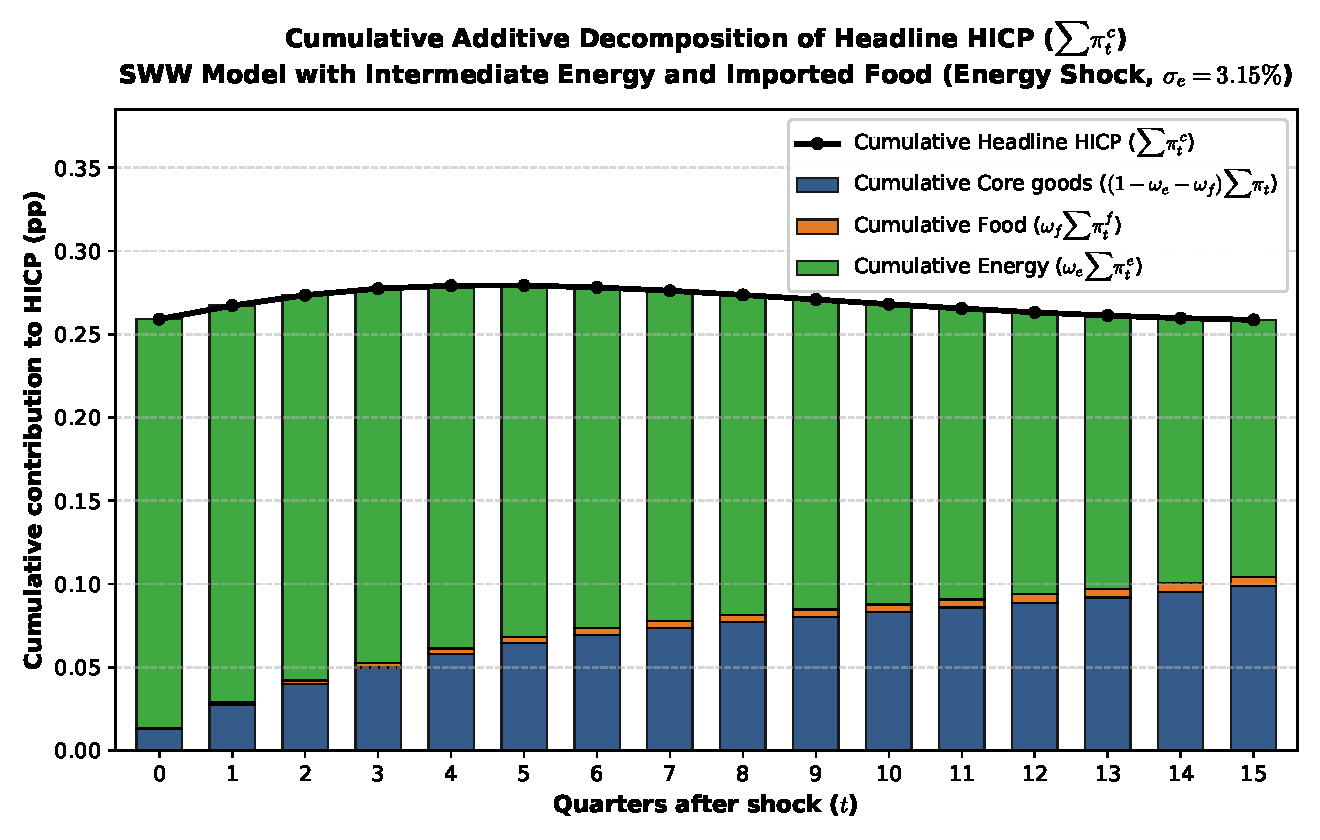
\includegraphics[width=0.90\textwidth]{Tabele/wykres_2_IRF_szoku_energetycznego/figure_2b_irf_decomposition_food_model_energy_shock.pdf}
\par\smallskip
\footnotesize\raggedright \textit{Source:} Own calculations based on the extended SWW (2014) DSGE model with intermediate energy ($\nu = 0.05$) and imported food basket ($\omega_f = 0.05, \omega_e = 0.0775$). 
The chart presents the exact additive decomposition of the cumulative headline HICP inflation response: $\sum_{k=0}^t \pi^c_k = (1-\omega_e-\omega_f)\sum_{k=0}^t \pi_k + \omega_e \sum_{k=0}^t \pi^e_k + \omega_f \sum_{k=0}^t \pi^f_k$. 
On impact ($t=0$), energy accounts for $94.7\%$ ($+0.245$ pp) of the headline price increase. After one year ($t=4$), persistent cost-push transmission via intermediate production increases the contribution of core domestic goods to $20.8\%$ ($+0.058$ pp), illustrating the gradual emergence of second-round effects.
\end{figure}

% Alternative: Comparison between Model with Energy vs Model with Energy & Food
\begin{figure}[H]
\centering
\caption{Cross-model comparison of cumulative HICP decomposition following an energy price shock ($\eta^e_t$).}
\label{fig:cumulative_irf_decomposition_comparison}
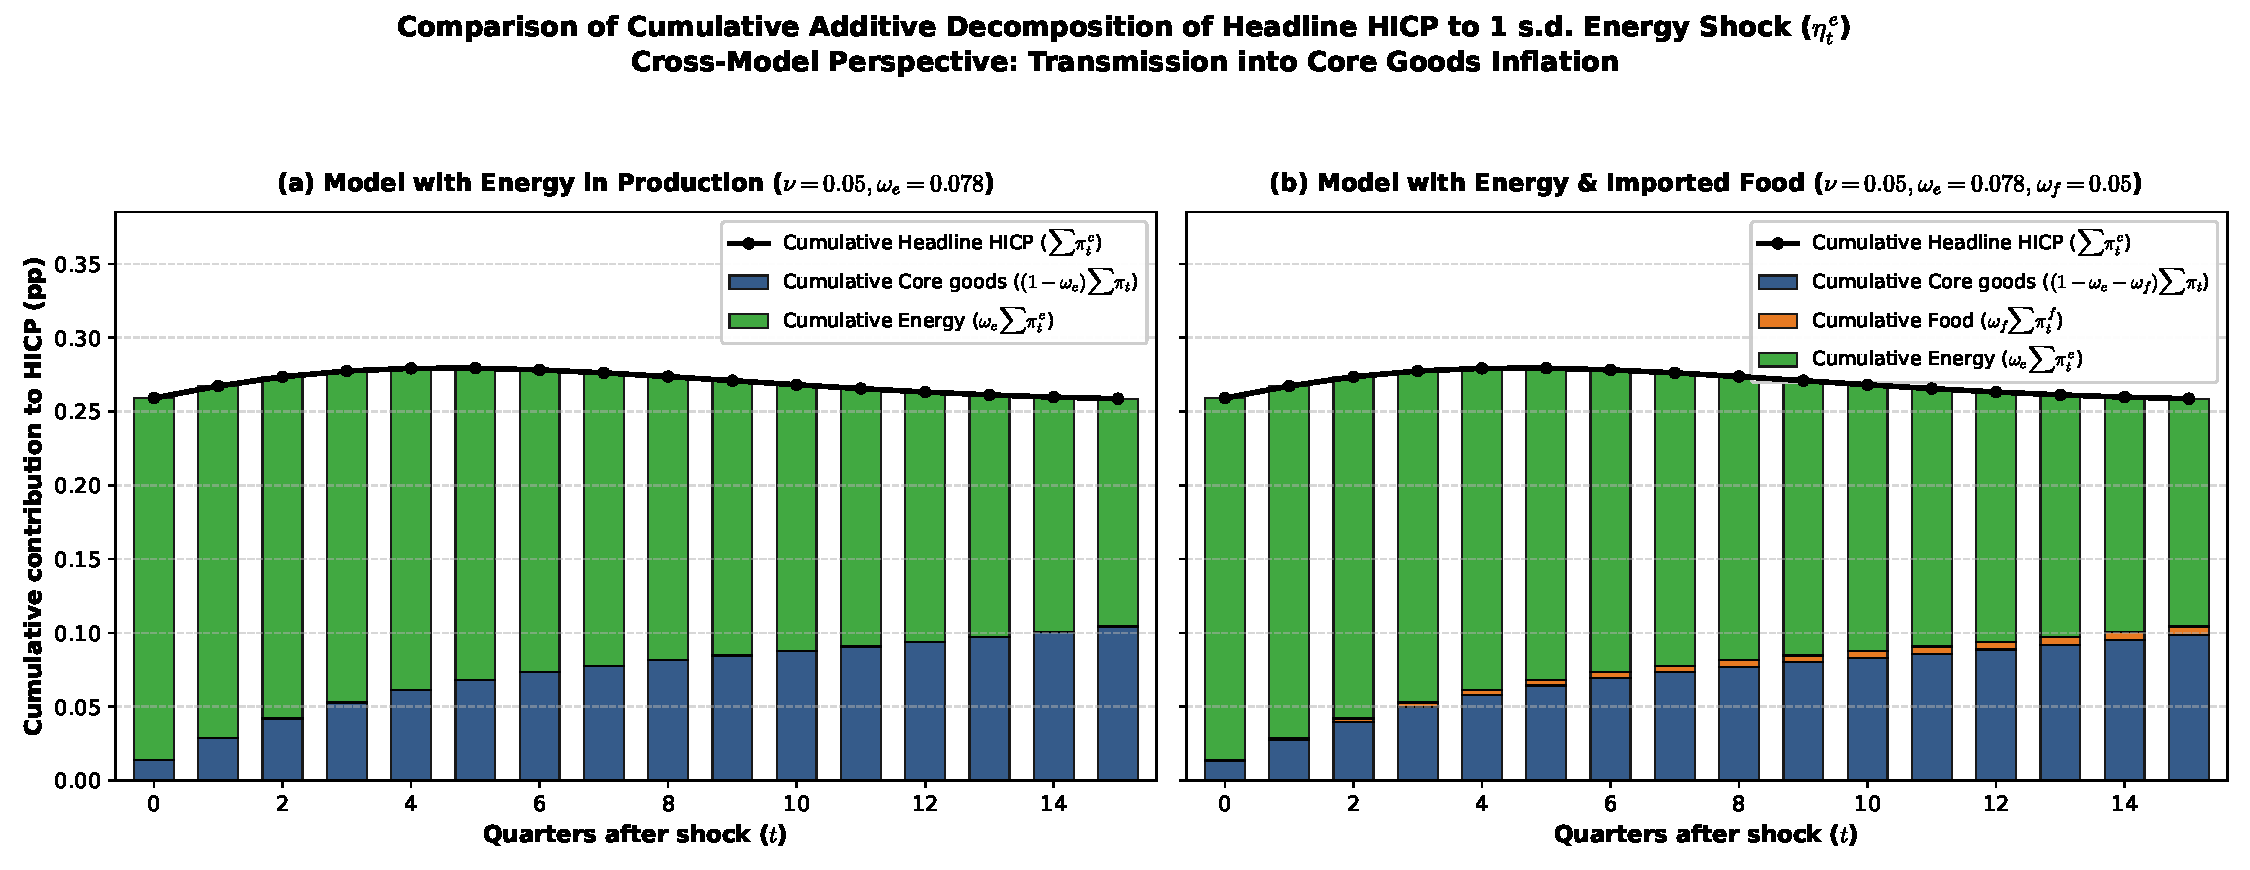
\includegraphics[width=0.98\textwidth]{Tabele/wykres_2_IRF_szoku_energetycznego/figure_2_comparison_energy_vs_food_models.pdf}
\par\smallskip
\footnotesize\raggedright \textit{Source:} Own calculations. Panel (a) shows the model with energy in intermediate production only ($\nu=0.05, \omega_e=0.0915$). Panel (b) shows the extended model with both intermediate energy and an imported food basket ($\omega_f=0.05, \omega_e=0.0775$).
\end{figure}
